\documentclass[12pt,a4paper]{article}
\usepackage{spex450_documents}

\title{Understanding MATLAB scripts and functions}

\author{Peter Lamb}

\date{Week 3}

\definecolor{OliveGreen}{RGB}{34 139 34}

\begin{document}

\maketitle


\section{Scripts}
A MATLAB script is simply a list of commands or instructions.  
Script files are saved as text files with the file extension \textbf{.m} to associate them with MATLAB.

\subsection{Executing a MATLAB script file}
An example script file has already been created and can be found in:
\begin{lstlisting}[style=Matlab-editor]
3-Scripts_and_functions\code.
\end{lstlisting}
Browse to this folder and then load the script file called `emgscript.m' into the \textbf{Editor}. %\footnote{It's common in Windows for the \textbf{.mat} extension to, by default, be associated with the Microsoft Access Table program, so if you try to open a \textbf{.mat} file from Windows Explorer you might launch a different program. If that happens, open the file from within MATLAB}. 
The commands that make up this script should look familiar from the previous chapter.  
We can use this file to run all of these commands at once.  
Make sure `3-Scripts\_and\_functions' is your \textbf{Current Folder} (more on this later); from within the \textbf{Editor} window click the \textbf{Run} icon from the toolbar.
If a dialog box opens, click \textbf{Add to Path} rather than \textbf{Change Folder}.  
You should see a figure appear containing the plot we produced in the previous chapter.  
%The script can also be run by typing the name of the script in the \textbf{Command Window} (without the \textbf{.m} bit) and pressing enter.  
%For example:
%\begin{lstlisting}[style=Matlab-editor]
%>> emgscript
%\end{lstlisting}

Because we have seen the commands before the script should make sense to us.  
However, someone who saw the script and those commands for the first time may find the code a bit confusing.  
MATLAB allows us to add text to these files that will not perform any actions.  
Putting the \textcolor{OliveGreen}{\%} character at the beginning of a line instructs MATLAB to ignore any following text it finds on the same line.  
This enables us to add a description/comment above a single or group of commands to remind us what is going on.  
Have a look at the file called `emgscriptwithdescription.m' to see how comments can make a file easier to understand.

\subsection{Creating your own MATLAB script file}
\label{sec:script}
We will now modify the existing script file to plot the first three of the EMG signals, each in a separate plot but within the same figure – a subplot.  
When MATLAB executes the \textbf{plot} function it draws the requested plot in the currently activated axis.  
If no axis has been created and activated, say after a blank figure has been created using the \textbf{figure} command, MATLAB draws the plot in a new axis.  
In order to create a number of plots within the same figure we can use the \textbf{subplot} command to create a series of new axes into which we can draw the required plots. %(note: \textbf{subplot} is a simplified implementation of the more customisable \textbf{axis} command. See the help documentation for more information).

\subsubsection*{Exercise}
\begin{enumerate}
	\item Use MATLAB's help documentation to find out how to use the \textbf{subplot} function.	
	\item Save a copy of the file `emgscriptwithdescription.m' and use this as the base for the following additions.  Choose any file name you like.
	\item Before the first plot on line 33, add a \textbf{subplot} command to specify that the figure should have a 3 row, 1 column arrangement and to plot into the first axis.
	\begin{itemize}
		\item Type the following:
		\begin{lstlisting}[style=Matlab-editor]
subplot(3,1,1);
		\end{lstlisting}	
		\item Add a comment above the \textbf{subplot} command to describe what action is being performed.
		\begin{lstlisting}[style=Matlab-editor]
% Setup the figure to have subplots arranged 
% in 3 rows and 1 column and then activate 
% subplot 1
		\end{lstlisting}		
	\end{itemize}
	\item Repeat this process to plot the next two signals in the second and third slots in the figure.
	\begin{itemize}
		\item Type the following:
		\begin{lstlisting}[style=Matlab-editor]
% Activate the second subplot in the 
% arrangement
subplot(3,1,2);

% Plot the EMG signal 2 against time and add 
% axis labels and a title
plot(emgdata(:,1), emgdata(:,3));
xlabel('Time (s)');
ylabel('EMG amplitude (mV)');
title('The EMG amplitude of signal 2');

% Activate the third subplot in the arrangement
subplot(3,1,3);

% Plot the EMG signal 3 against time and add 
% axis labels and a title
plot(emgdata(:,1), emgdata(:,4));
xlabel('Time (s)');
ylabel('EMG amplitude (mV)');
title('The EMG amplitude of signal 3');
		\end{lstlisting}		
	\end{itemize}
	\item Run this new script (in my case I called it `myscript.m'), either by clicking the \textbf{Run} button from the toolbar of the \textbf{Editor}.
	\begin{lstlisting}[style=Matlab-editor]
>> myscript
	\end{lstlisting}
\end{enumerate}

\begin{figure}[H]
\begin{center}
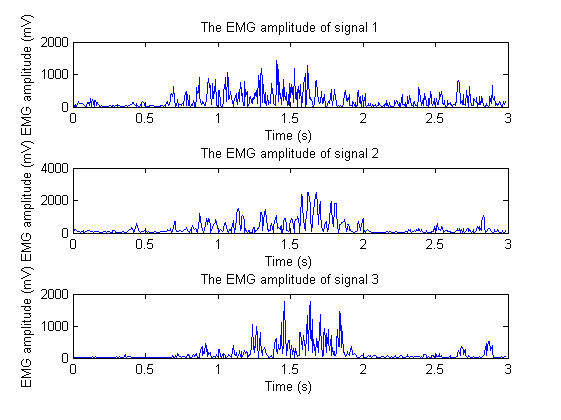
\includegraphics[width=\textwidth]{script_output.png}
\caption{A figure showing three subplots of the first three EMG signals}
\label{fig:scriptoutput}
\end{center}
\end{figure}

\section{Functions}
We have already had some experience in using MATLAB's in-built functions.  
Let us now take a closer look at how these functions work.  
However, in order to get a good look at how these functions work we will have to look at a function that is not an in-built one.  
This is because all of the code in MATLAB functions is hidden.  
Take a look at the file `my\_abs.m' in the `code' subfolder, which contains the function \textbf{my\_abs}.  
The aim of this function is to perform exactly the same operation as MATLAB's \textbf{abs} function that we have used previously.

As you can see, this function appears similar in many ways to the \textbf{scripts} we have just been using.  
However, there are some fairly significant differences.  
The main thing to notice is that the function is defined at the start of the file using the command \textbf{function}.  
This is a requirement and this line must be the first command that MATLAB encounters (ignoring any comments).  
The function declaration for the example in `my\_abs.m' is the following:
\begin{lstlisting}[style=Matlab-editor]
function abs_data = my_abs(input_data)
\end{lstlisting}
This line instructs MATLAB in a few ways.
\begin{itemize}
\item It instructs MATLAB that what follows is a function.
\item It declares an output variable called \textbf{\texttt{abs\_data}}.  This instructs MATLAB that at the end of the function it should return the value contained in the variable \textbf{\texttt{abs\_data}}.
\item It states the name of the function, in this case \textbf{\texttt{my\_abs}}.
\item It creates a variable called \textbf{\texttt{input\_data}}.  This will be the value that is passed to the function when it is called.  For example if we call the function \textbf{\texttt{my\_abs}} by typing:
\begin{lstlisting}[style=Matlab-editor]
>> testdata = my_abs(emgdata);
\end{lstlisting}
then within the function the variable \textbf{\texttt{input\_data}} would be exactly the same as the variable \textbf{emgdata}.
\end{itemize}

Try using this function as we have before by typing\footnote{More on the line \textbf{\texttt{addpath('code')}} later}:
\begin{lstlisting}[style=Matlab-editor]
>> addpath('code')
>> testdata = my_abs(emgdata);
\end{lstlisting}
Notice how we only see the variable \textbf{testdata} appear in the \textbf{Workspace} and not any of the intermediate variables e.g.~\textbf{\texttt{squared\_data}} or \textbf{\texttt{square\_root\_squared\_data}}.  
This is one of the main benefits of a function.  
However, in the same way that we do not see any of the function variables in the workspace, we also do not see any of the workspace variables in the function.  
The only workspace variables that can be used in the function are the variables that are passed into the function.  
Similarly, the only function variables available back in the workspace are the ones returned from the function.  
All clear!?  
If not, try not to worry too much, that is about as complicated as things will get with function use and you will see and experience many more examples of these principles.

\subsection{Writing your own functions}
Using all of the skills we have gathered so far we will write a new function called \textbf{rectify} that will rectify EMG signals.  
MATLAB has a tool that will help to create the template of a function automatically.  
Either in the \textbf{Home} tab or the \textbf{Editor} window, click the dropdown arrow under \textbf{New} and choose \textbf{Function}.  
For now we will assume that the input to the \textbf{rectify} function is just a single column vector.

\subsubsection*{Exercise}
\begin{enumerate}
	\item Create a new Function and name the function \textbf{rectify}
	\begin{itemize}
		\item From the \textbf{Home} tab on MATLAB ribbon select \textbf{New} and then from the drop down list select \textbf{Function}.
		\item MATLAB will create a new file and add the required code and an example function name.  
		Change the function name (declared on the first line of the new file) from \textbf{Untitled} to \textbf{rectify}.
		\item Change the function input and output variables to more meaningful names.  E.g. \textbf{\texttt{raw\_emg}} as the input and \textbf{\texttt{rectified\_emg}} as the output (just helps with readability).
		\item Replace the function comments with a brief description of what we are trying to achieve.
		\item Click the \textbf{save} button.  Choose the \textbf{code} folder (Notice how MATLAB has already chosen the name of the file as `rectify.m').  Click \textbf{Save}.
	\end{itemize}
	\item As we are creating this function look at some of the ways that the \textbf{Editor} helps us.
	\begin{itemize}
		\item Notice how the input and output variables are underlined in orange.  The bar to the right of the window has an orange square and a line next to the function declaration.
		\item Try hovering the mouse icon over the underlined text and see what information MATLAB gives us.
		\item It tells us that one variable is not used (\textbf{\texttt{raw\_emg}}) and the other is unset (\textbf{\texttt{rectified\_emg}}).
		\item Orange underlining is MATLAB's way of letting us know that although the code may work we may be in need of some helpful warnings.
		\item Red underlining lets us know that MATLAB has encountered some commands that will not work and will result in errors.
		\item Try typing something ridiculous and see if you can get the \textbf{Editor} to give you some red writing.
		\item Remember to delete your nonsense!
	\end{itemize}
	\item Add the commands that will baseline correct and rectify the signal.
	\begin{itemize}
		\item The function \textbf{mean} will calculate the average value of the signal.  This can be used to baseline correct.
		\begin{lstlisting}[style=Matlab-editor]
baseline = mean(raw_emg);
baseline_corrected_emg = raw_emg-baseline;
		\end{lstlisting}
		\item The function \textbf{abs} will calculate the absolute value of the signal.  This can be used to rectify.
		\begin{lstlisting}[style=Matlab-editor]
rectified_emg = abs(baseline_corrected_emg);
		\end{lstlisting}			
	\end{itemize}
	\item Hopefully you should see a green square at the top of the right hand border to indicate that no warnings or errors have been found.	
	\item Click the \textbf{save} button to save your changes.
	\item Test out the function with a column from the variable \textbf{datacsv}.
	\begin{itemize}
		\item Plot some raw data from \textbf{datacsv}
		\begin{lstlisting}[style=Matlab-editor]
>> plot(datacsv(:,2));
		\end{lstlisting}
		\item Rectify the same raw data
		\begin{lstlisting}[style=Matlab-editor]
>> testdata = rectify(CSVData(:,2));
		\end{lstlisting}	
		\item Plot the new rectified data
		\begin{lstlisting}[style=Matlab-editor]
>> plot(testdata);
		\end{lstlisting}	
		\item Depending on which column you decided to plot you should see something like this:
		\begin{center}
			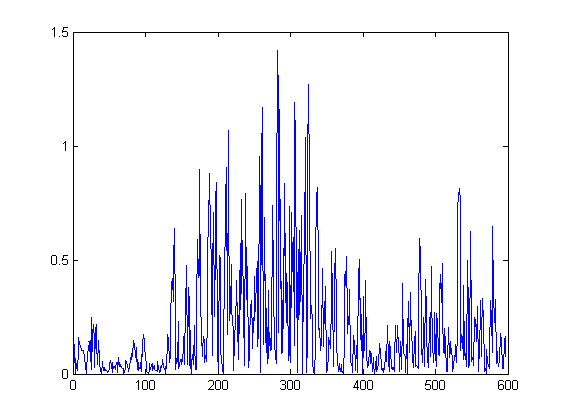
\includegraphics[width=\textwidth]{csvdata2rectified.png}
		\end{center}
	\end{itemize}	
\end{enumerate}

\end{document}